\chapter{Characteristics of the cloud service HPC used}
\section{Introduction}
The HPC used in this thesis to run all the test scenarios is a cloud service based HPC.
NVIDIA offers in a collaboration with Matlab and Amazon: the MATLAB Deep Learning Container on NVIDIA GPU Cloud.
Where the NVIDIA GPU Cloud is hosted by Amazon Web Services or AWS.
\par 
In AWS the user can run virtual machines on the amazon cloud and access these virtual machines from home.
These virtual machines are based on starting image files, called AMIs.
The AMI used in this thesis is called: NVIDIA Deep Learning AMI.
\par
As earlier described the virtual machine used is actually an ubuntu os with a docker container on top.
Matlab runs in this docker container.
I put up a secure ssh tunnel from the virtual machine to my personal device, mapping ports from the virtual machine to my personal sockets.
This allowed me to work in the docker container from my personal computer web browser.
File transfer is integrated with the use of Matlab Drive, making it very easy to make alterations on both my personal device and the virtual machine.
\section{Characteristics and performance}
As shown in figure~\ref{fig:awsspec}, the CPU is an Intel Xeon E5 and the GPU a NVIDIA Tesla V100 SXM2.
According to NVIDIA the fastest GPU in the world.\cite{NVIDIAV181:online}
A benchmark run gave the following results:
\begin{figure}[H]
	\centering
	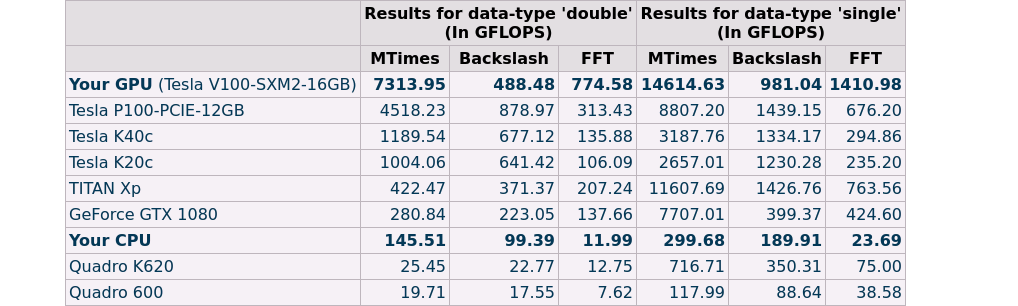
\includegraphics[width=\linewidth]{benchmark1.png}
	\caption{MATLAB Deep Learning Container on NVIDIA GPU Cloud Benchmark Overview.}
\end{figure}
\begin{figure}[H]
	\centering
	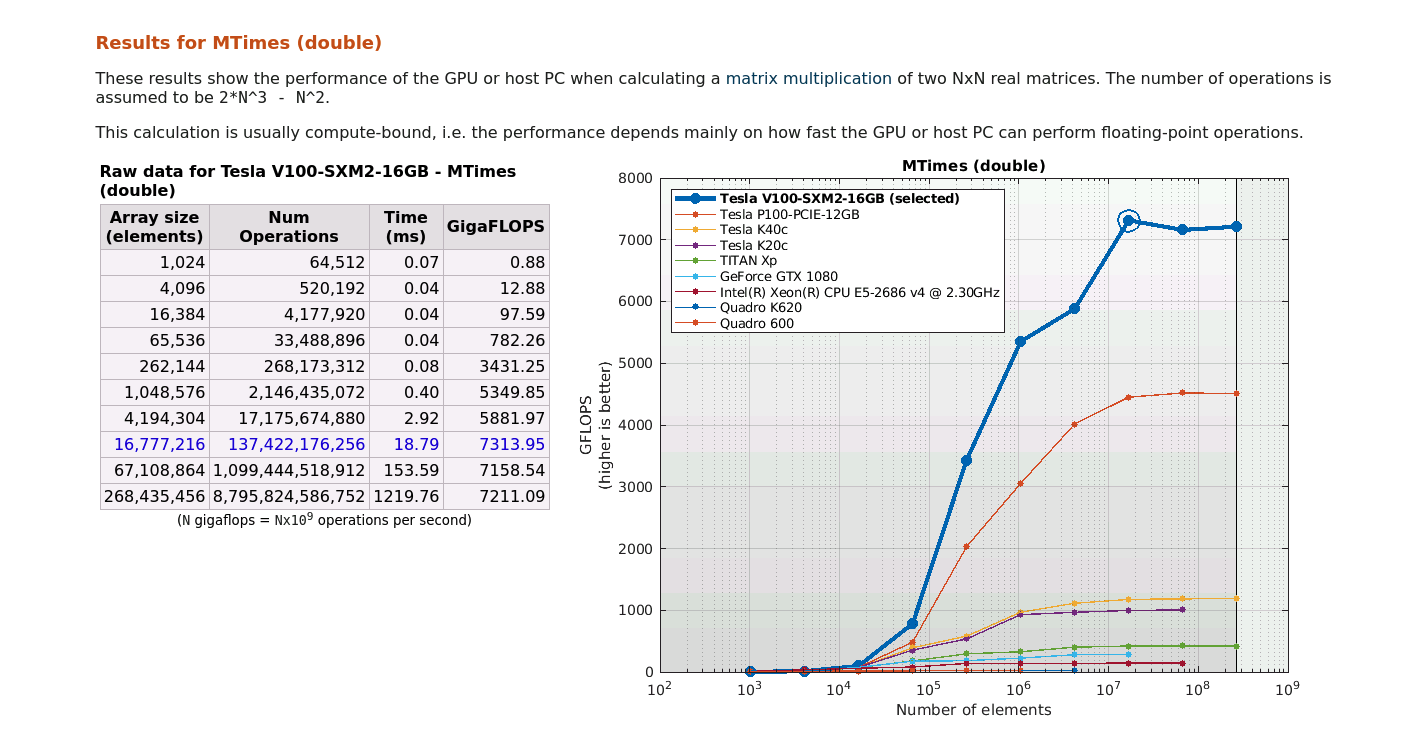
\includegraphics[width=\linewidth]{benchmark2.png}
	\caption{MATLAB Deep Learning Container on NVIDIA GPU Cloud Benchmark MTimes (double).}
\end{figure}
\begin{figure}[H]
	\centering
	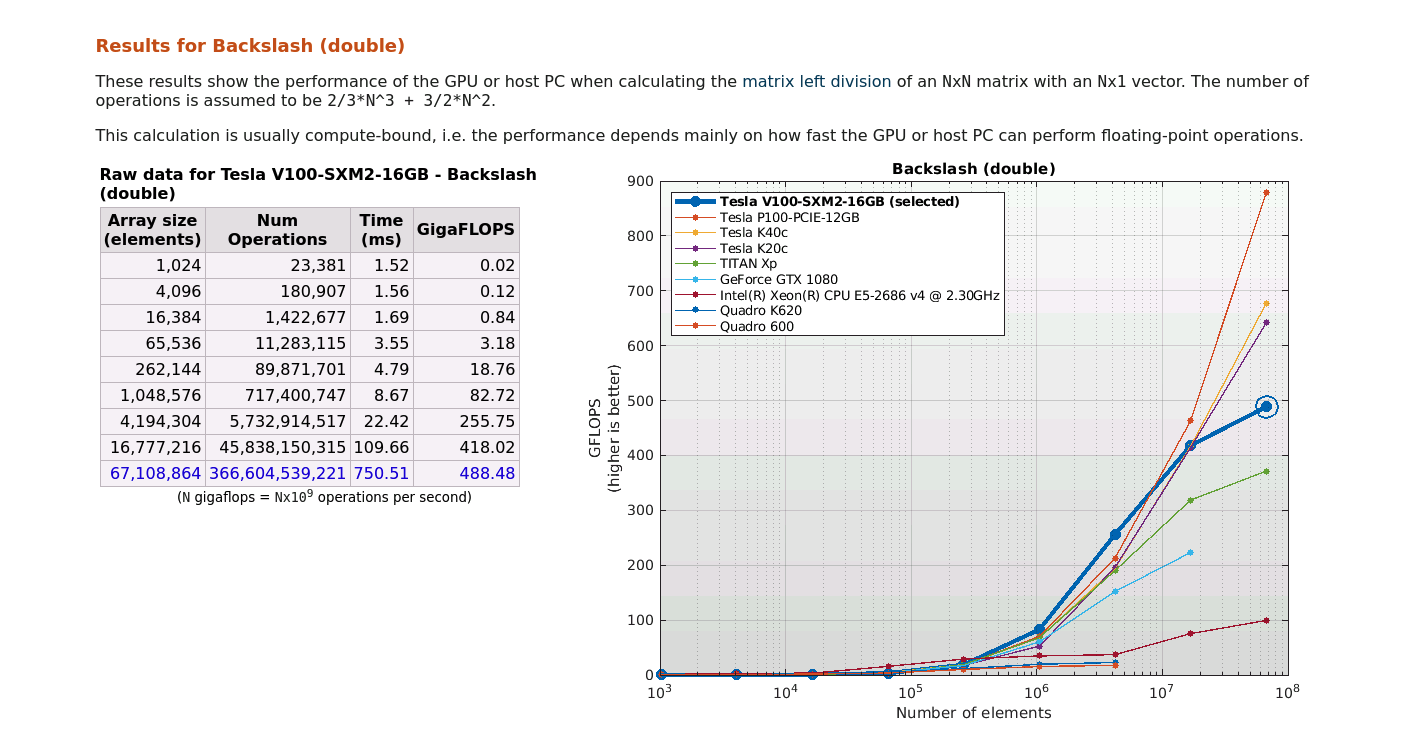
\includegraphics[width=\linewidth]{benchmark3.png}
	\caption{MATLAB Deep Learning Container on NVIDIA GPU Cloud Benchmark Backslash (double).}
\end{figure}
\begin{figure}[H]
	\centering
	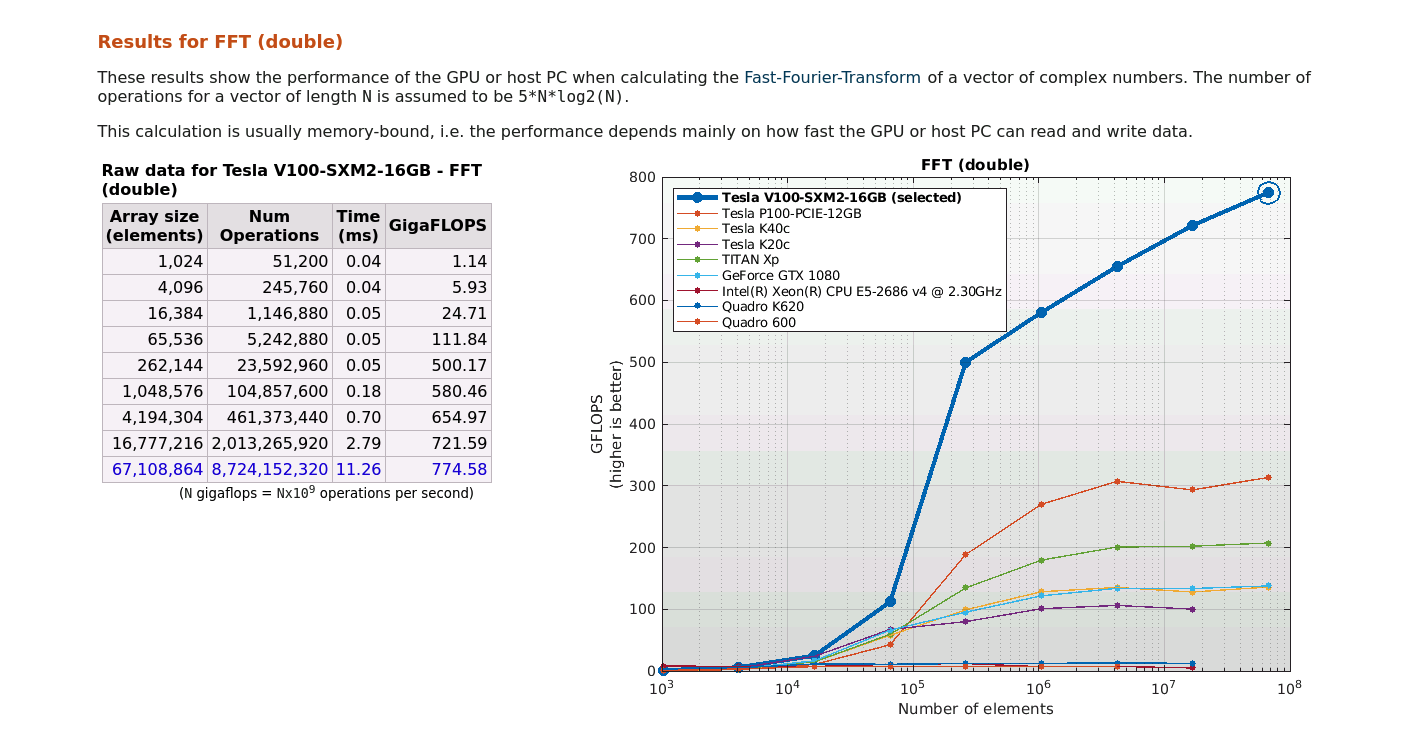
\includegraphics[width=\linewidth]{benchmark4.png}
	\caption{MATLAB Deep Learning Container on NVIDIA GPU Cloud Benchmark FFT (double).}
\end{figure}
\begin{figure}[H]
	\centering
	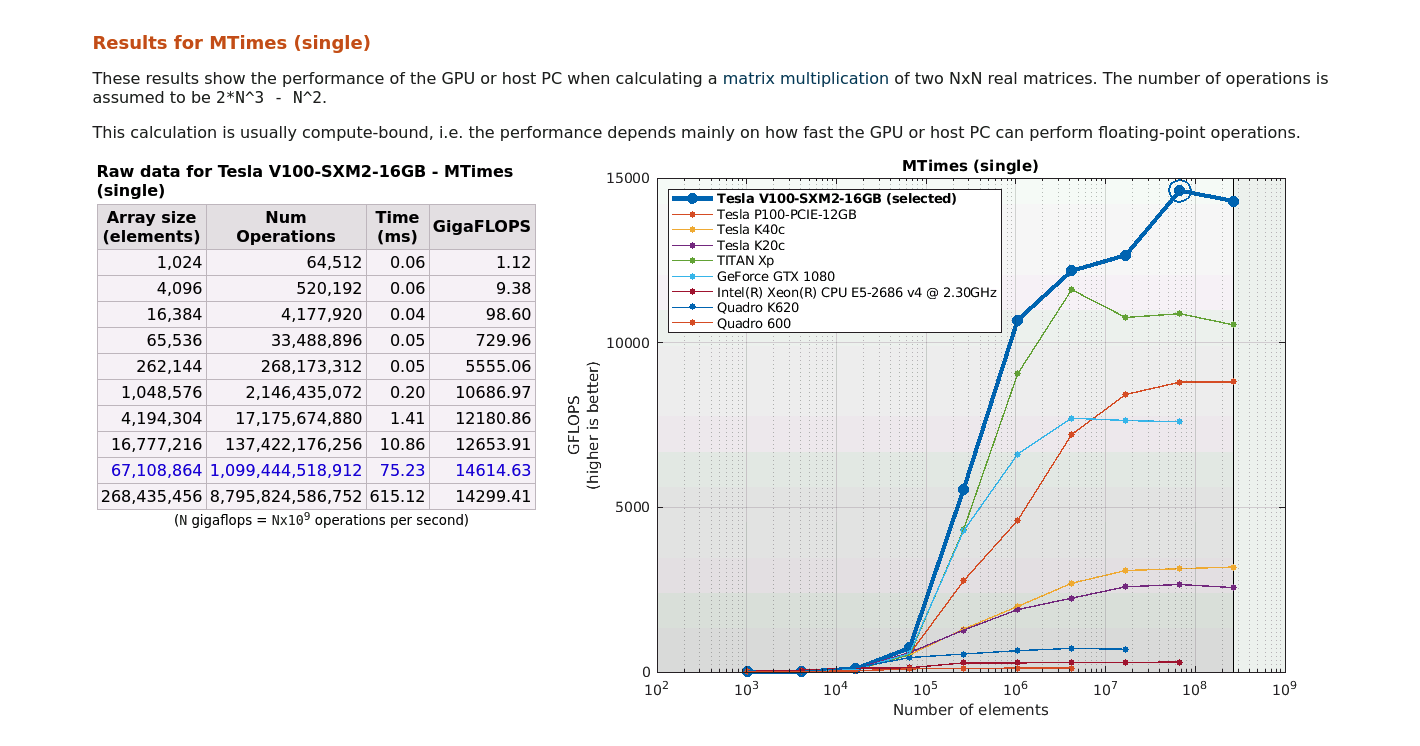
\includegraphics[width=\linewidth]{benchmark5.png}
	\caption{MATLAB Deep Learning Container on NVIDIA GPU Cloud Benchmark MTimes (single).}
\end{figure}
\begin{figure}[H]
	\centering
	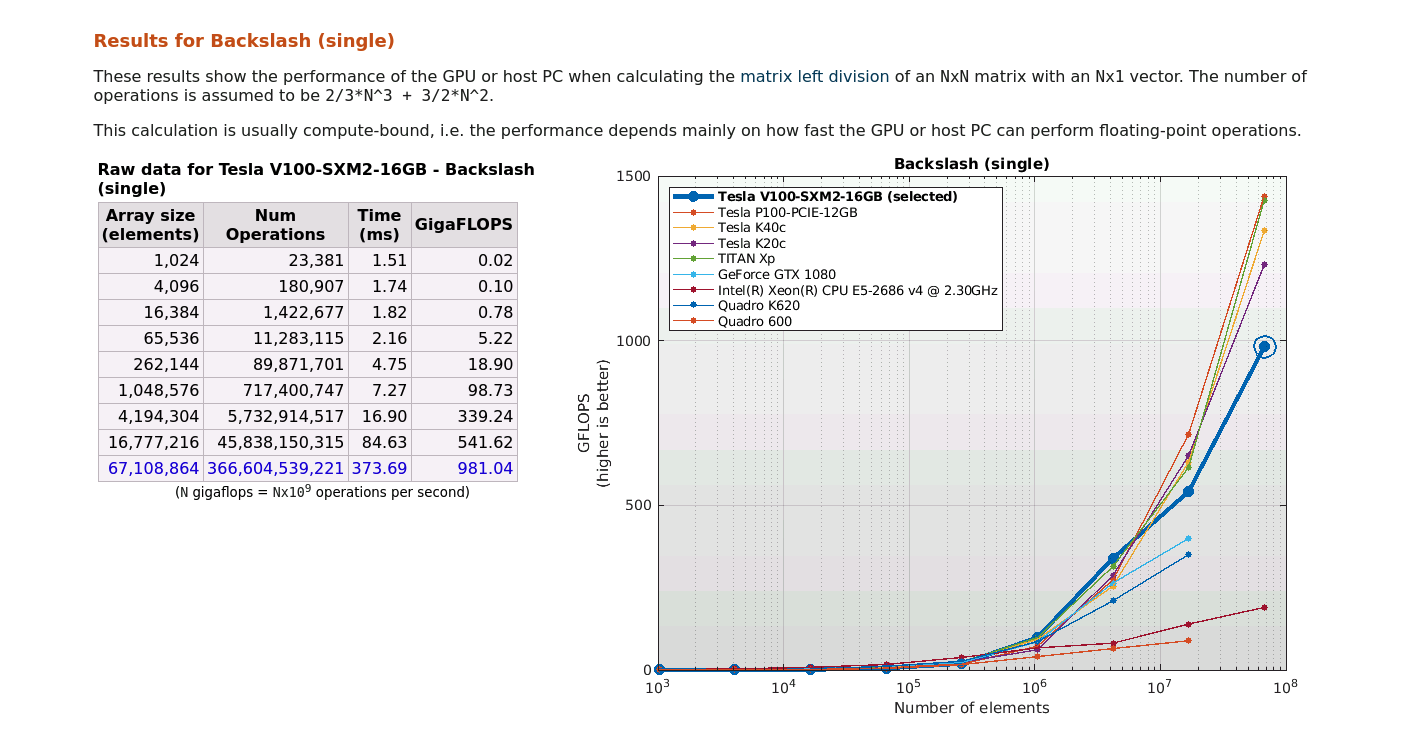
\includegraphics[width=\linewidth]{benchmark7.png}
	\caption{MATLAB Deep Learning Container on NVIDIA GPU Cloud Benchmark Backslash (single).}
\end{figure}
\begin{figure}[H]
	\centering
	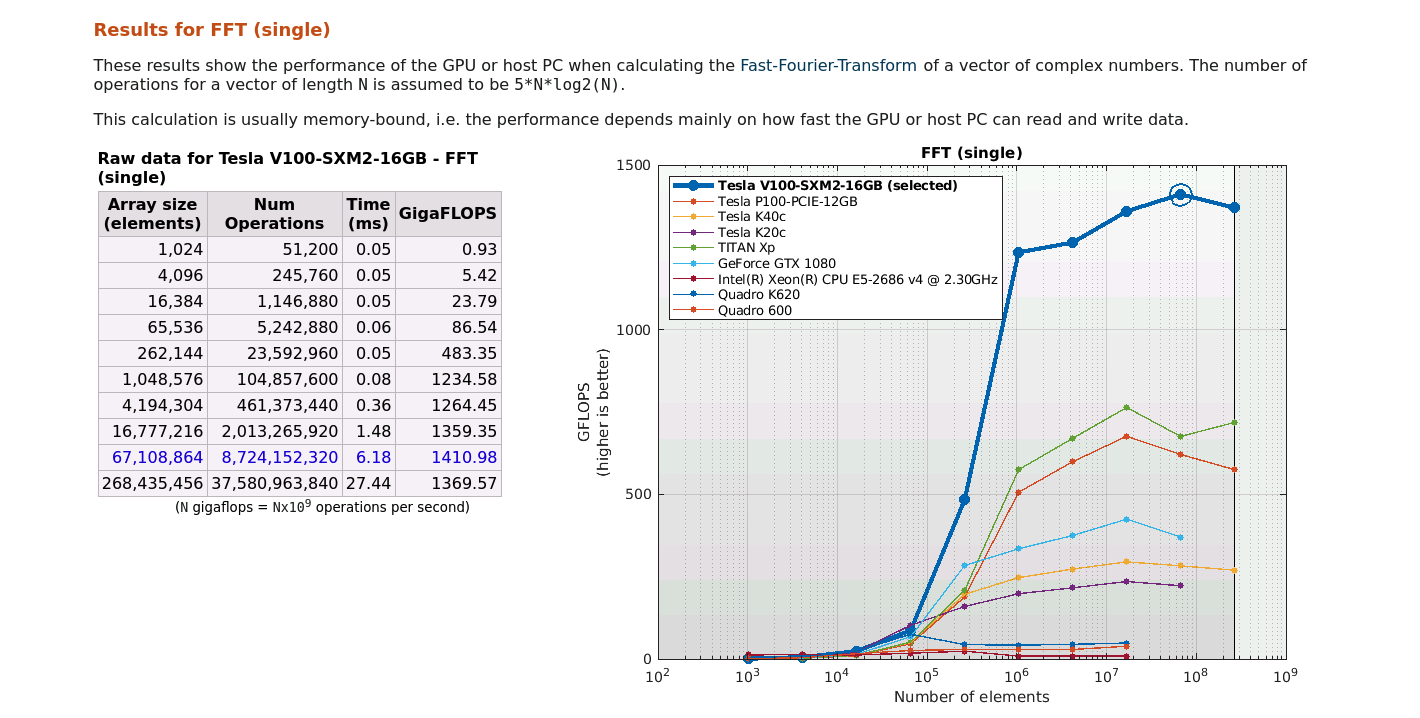
\includegraphics[width=\linewidth]{benchmark8.png}
	\caption{MATLAB Deep Learning Container on NVIDIA GPU Cloud Benchmark FFT (single).}
\end{figure}
\begin{figure}[H]
	\centering
	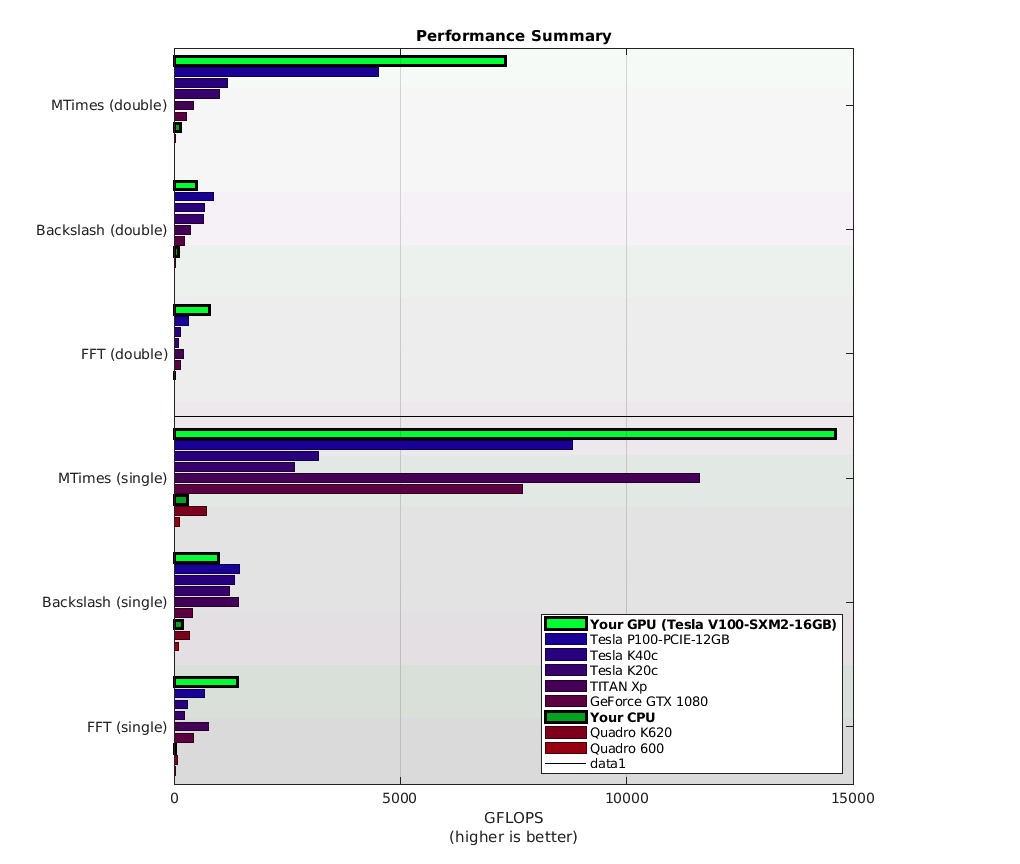
\includegraphics[width=0.8\linewidth]{benchmark9.png}
	\caption{MATLAB Deep Learning Container on NVIDIA GPU Cloud Benchmark Overview Diagram.}
\end{figure}